\chapter{Results}
\label{chap:results}
\section{Dredging activities}
This section describes the relevance of dredging to the sediment balance of the designated area, by an estimation of the dredging volumes through different data sources. It includes an analysis of the data gathered through interviews, through AIS data and extraction permits. 

\subsection{Stakeholder interviews}
During the fieldwork, ten interviews with stakeholders were conducted. Responses were recorded and these raw results are given in Appendix \ref{chap:interviews}. The nature of the dredging activities was addressed in almost all interviews. 

\subsubsection{Number of boats}
Stakeholders provided many insights on the scale and development of dredging in the Paraná Guazú river. The caretaker at the Fisher’s Club didn't perceive any increase in recent years, while nearby landowners recalled that the number of dredgers used to be higher, with only two remaining active today. The mayor of Ibicuy confirmed this trend, explaining that most dredging vessels left the Paraná Ibicuy after municipal taxes on sand extraction were raised. At the Port of Ibicuy, the administrator remembered that small dredgers, no longer than twenty meters, once handled sand but have since disappeared; dredging activities there have ceased altogether and moved to a different port (Port Constanza). A private dredger entrepreneur described his own ship, the Vizcaíno 978, which has been prepared for operation after years of administrative delay.

\subsubsection{Purpose of dredged sand}
Stakeholders also offered insights into the purposes for which dredged sand is used. According to the the mayor, river sand is generally used for construction materials and, in some cases, glass production. The port administrator confirmed that the sand once handled in Ibicuy was also directed toward the construction sector. The dredger entrepreneur described a mixed market, with sand used primarily for concrete, but also increasingly sold to the fracking industry when sufficiently fine-grained. The YPF mine manager confirmed that the company uses river sand for fracking purposes, although not necessarily from the area of interest.

Overall, stakeholders agreed that construction is the traditional destination of dredged sand. However, multiple stakeholders noted that demand for construction sand has declined in recent years, due to the slowdown of public building projects. In contrast, the demand for fracking sand has been growing steadily, as highlighted by the YPF manager. The dredger indicated that selling to YPF might be a viable option.

\subsection{Data analysis}
In addition to the stakeholder interview information, AIS data and extraction permits were studied to learn more about the dredging activities on the river. 
\subsubsection{Vessel positioning information (AIS)}
Using MarineTraffic it was found that two dredgers are operating on the Paraná Guazú between Ibicuy and Brazo Largo: the Comercio Segundo and the E.M. Arroyo N1. The Comercio Segundo has a length of 30 m, a width of 7 m, a draft of 1.3 m, and an approximate cargo hold of 195 m\textsuperscript{3}. The E.M. Arroyo N1 has a length of 39 m, a width of 8 m, a draught of 2.8 m and an approximate cargo hold of 476 \,m\textsuperscript{3}. Using a sand to water ratio of 3:1 for the dredged slurry, the amount of sand dredged is 150 \,m\textsuperscript{3} and 360 \,m\textsuperscript{3} respectively per cargo. The tracks of the two vessels obtained from MarineTraffic are shown in Figures 5.1 and 5.2.

\begin{figure}[H]
    \centering
    \begin{minipage}{0.48\textwidth}
        \centering
        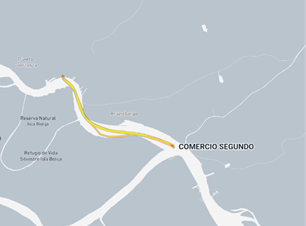
\includegraphics[width=\linewidth]{figures/ch5/Track_CS.png}
        \caption{Track of the \textit{Comercio Segundo}}
        \label{fig:track_cs}
    \end{minipage}\hfill
    \begin{minipage}{0.48\textwidth}
        \centering
        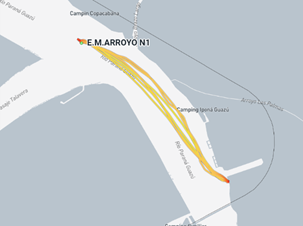
\includegraphics[width=\linewidth]{figures/ch5/Track_EM.png}
        \caption{Track of the \textit{E.M. Arroyo N1}}
        \label{fig:track_em}
    \end{minipage}
\end{figure}

The AIS data for these two vessels is obtained from MyShipTracking, which is used to determine the location of the dredging and the average number of trips. The dredging location of the two vessels is shown in Figure 5.3. It can be seen that both dredgers dredge in the same area. This can be explained by the bathymetry shown in Figure 5.4, which shows a reduced depth near the junction of the two navigable channels. At this location the flow velocity is lower, causing sediment to settle and thus creating a sandbar. From the AIS data it can be concluded that both dredgers make three trips per day.

\begin{figure}[H]
    \centering
    \begin{minipage}{0.48\textwidth}
        \centering
        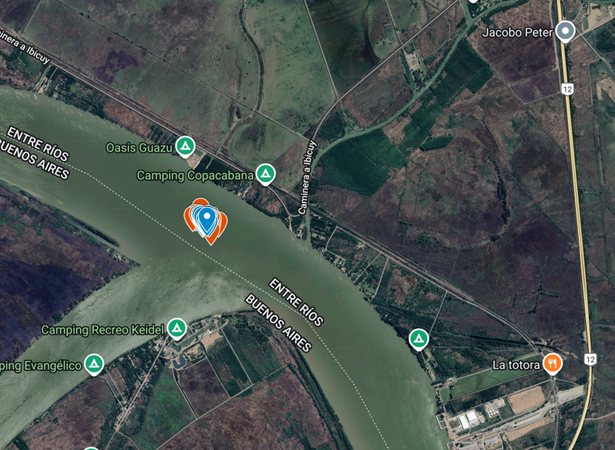
\includegraphics[width=\linewidth]{figures/ch5/Dredging_coordinates.png}
        \caption{Dredging location}
        \label{fig:dredging_coordinates}
    \end{minipage}\hfill
    \begin{minipage}{0.48\textwidth}
        \centering
        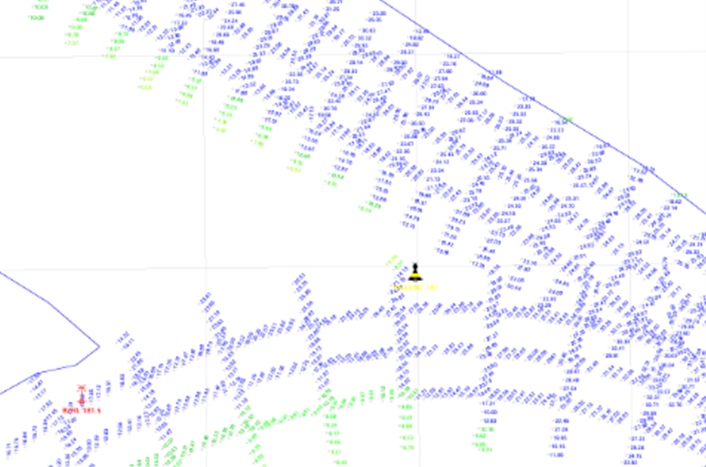
\includegraphics[width=\linewidth]{figures/ch5/Bathymetry.png}
        \caption{Bathymetry}
        \label{fig:bathymetry}
    \end{minipage}
\end{figure}

In the Rio Talabera, a side branch connecting to the Paraná Guazú, a third dredger is extracting sand. The Altair is dredger with a length of 66 m, a width of 11 m, a draught of 1.5 m and a approximate cargo hold of 750 \,m\textsuperscript{3}. Using the same sand to water ratio of 3:1 this gives 560 \,m\textsuperscript{3} of sand per cargo. Using MarineTraffic it was found that the Altair has an average 3 trips per day. Figure 5.5 shows the track of the Altair and the location at which it stops to extract sand. 

\begin{figure}[H]
    \centering
    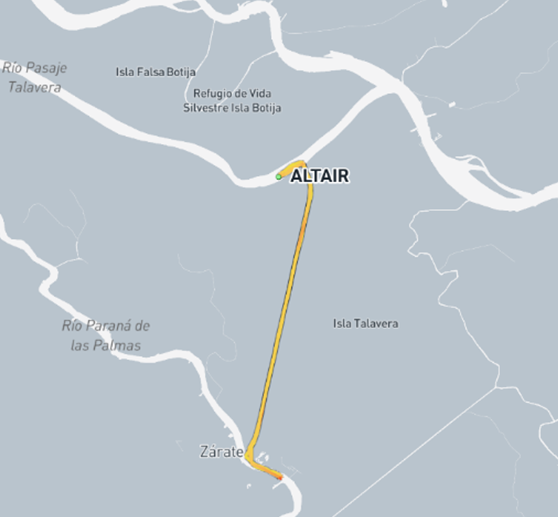
\includegraphics[width=0.5\linewidth]{figures/ch5/Track_Altair.png}
    \caption{Track of the Altair}
    \label{fig:placeholder}
\end{figure}

For all three vessels, the estimated volume of sand extracted per month is displayed in table 5.1
\begin{table}[h!]
\centering
\begin{tabular}{lrrrr}
\hline
\textbf{Vessel} & \textbf{Cargo hold} & \textbf{Sand volume [\,m\textsuperscript{3}]} & \textbf{Trips per day} & \textbf{Volume per month [\,m\textsuperscript{3}]} \\
\hline
Comercio Segundo & 195 & 150 & 3 & 9000 \\
E.M. Arroyo N1 & 476 & 360 & 3 & 21600 \\
Altair & 750 & 560 & 3 & 33600 \\
\hline
\end{tabular}
\caption{Sand transport details per vessel.}
\label{tab:sand_volume}
\end{table}

\subsubsection{Extraction permits}
A total of 33 permits were collected for the Paraná Guazú and 43 for the Ibicuy. On the Paraná Guazú, four permits were issued for channel maintenance, while the remainder concerned sand extraction. For the Ibicuy, all permits were related to extraction activities. The analysis shows that the requested volumes in the Ibicuy are considerably larger than those in the Paraná Guazú, even though the section of the Ibicuy considered here is much shorter in length.

It is important to note that the end dates of contracts are unknown. While the requests specify monthly dredging quantities, they do not indicate the duration of the works. As a result, a detailed quantitative assessment cannot be made. For the present analysis, all requests with fixed monthly volumes are assumed to extend over 12 months, allowing for a comparison between the two river sections, as shown in Figure \ref{fig:yearly dredging volumes}. The second assumption is to record a single value for the requested volume, when information about monthly or yearly occurrence is lacking.

\begin{figure}[H]
    \centering
    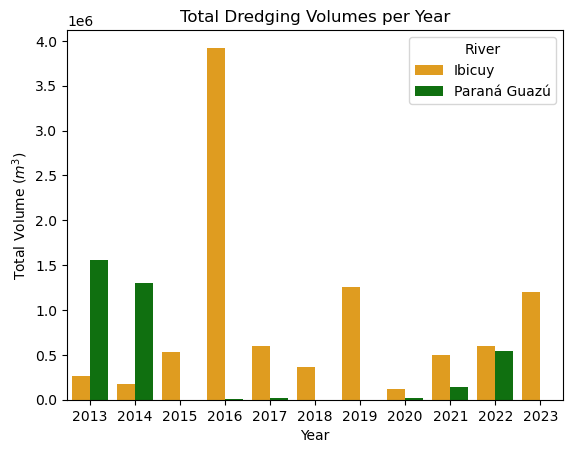
\includegraphics[width=0.50\linewidth]{figures/ch2/Dredging volumes permits.png}
    \caption{Yearly dredging volumes}
    \label{fig:yearly dredging volumes}
\end{figure}

\subsection{Estimated sand extraction}
This section draws a conclusion on the sand extraction volumes, such that an estimate is found to apply in the sediment balance. The following uncertainties were considered in determining a representative value:

\begin{itemize}
    \item Not every vessel in the area is equipped with an AIS transponder, meaning that possibly not all active vessels were identified. However, the number of vessels as found by analysis of the AIS data was in agreement with the number of vessels as observed during the fieldwork.
    \item No historical AIS data was available, such that the data was registered for only a short period of time.
    \item The extraction permits do not mention the duration of the contract.
\end{itemize}

However, a rough estimate can be found by calculating the mean annual volume for the total system of interest (i.e., Ibicuy and Paraná Guazú). To make a comparison with the monthly values in Table \ref{tab:sand_volume}, this yearly value is reduced to a monthly value by dividing by 12 months. The former approach yields the following value for dredged sand volumes:

\begin{equation}
    V_{sand,yearly} = 1193923 ~m^3
\end{equation}
\begin{equation}
    V_{sand,monthly} = \frac{V_{sand,yearly}}{12} \approx 100000 ~m^3 
\end{equation}

\section{Effects of dredging}
This study aims to examine the effects of dredging on the river, with a focus on its ecological and geomorphological impacts. These impacts were explored through a combination of stakeholder interviews and data analysis.

\subsection{Stakeholder interviews}
Stakeholders expressed contrasting views on the ecological and geomorphological impacts of dredging in the Paraná Guazú. Mostly the impacts on fish populations and bank stability were discussed.

\subsubsection{Fish populations}
The caretaker of the Fisher’s Club reported a noticeable decline in fish populations. He did not link this directly to the dredging activities, but instead pointed to contamination from agricultural fertilizers. In contrast, a municipal representative from Zárate questioned the narrative of decline, arguing that complaints about fewer fish reflect generational shifts among fishers rather than an actual reduction.

\subsubsection{Riverbank stability}
When it comes to riverbank stability, landowners described severe erosion of up to thirty metres per year, which they attributed to the activities of dredging vessels and passing cargo ships. The caretaker added that vegetation removal near the club increased local erosion. In contrast to this, the mayor of Ibicuy downplayed the role of dredging, attributing bank collapses in his jurisdiction to the natural flow of the river. Futher, in 2011 there was a qual wall collapse in the Port of Ibicuy, but the portmanager claimed that this was an accident and not due to the sand extraction activities.

\subsection{Data analysis}
Hier hydraulic analyse?
Onderbouwing van wrm baggeren niet zoveel effect heeft

\section{Dry sand mining}
The practice of dry sand mining and its effects were also researched. In this section, the results from both stakeholder interviews and data analysis are presented for the dry sand mining activities. 
\subsection{Stakeholder interviews}
The significance of dry sand mining activities emerged from stakeholder interviews and field observations. The interview results are given first.
\subsubsection{Extent}
Stakeholders consistently underlined the large scale and rapid growth of dry sand mining in the region. The caretaker at the Fisher’s Club estimated that around 500 trucks leave the area each month carrying 40–45 tons of sand each, noting that this number has doubled compared to when he started his job 4.5 years ago. The mayor of Ibicuy described an even larger scale, reporting that approximately 350 trucks transport some 9,000 tons of sand daily. These impressions were confirmed by the YPF plant manager, who stated that his mine alone extracts about 120,000 tons of sand per month and that output is expected to increase in the coming years. He also referred to geological surveys indicating sufficient reserves to sustain regional extraction for 88 years. This number was confirmed by the mayor, who added that in areas of intense extraction this would be around 40 years.

\subsubsection{Effects}
Multiple effects of these activities were named by interviewees. The caretaker observed that waste from washing processes flows back into the river, making the water dirtier, while the removal of sand on land reduces drainage capacity and therefore increases flooding risks. He and the mayor both emphasized the damage caused by heavy truck traffic, which worsens road conditions and leads to complaints from locals. The mayor added that judicial interventions have forced authorities to introduce extraction limits and monitoring mechanisms, as uncontrolled mining had raised public concerns.

\subsubsection{Purpose}
Stakeholders emphasized that the dominant purpose of dry sand mining in the region is to supply the fracking industry. Both the mayor, port administrator, dredger and the Fisher's club caretaker indicated that most or all dry sand is sold to YPF.

The YPF plant manager explained that the sand extracted is transported primarily to Añelo, in the province of Neuquén, where it is used in fracking operations. He highlighted that this sand is very rich in quarts, is fine-grained and highly resistant, which makes it well-suited for use as proppant, to keep fractures in the shale open during extraction. According to him, these properties are not easily substituted by sand from different locations or other alternatives.

Some stakeholders recalled that also the dry sand was traditionally associated with construction or in some cases glass production, but they acknowledged that these markets have become secondary to the fracking. Part of this is the decreasing demand for construction sand. The port administrator, the YPF mine manager and the dredger all indicated that demand from construction has declined due to the reduction of public building projects. The demand for sand to be used in fracking, on the other hand, is constant according to the dredger and is even increasing according to the YPF manager.

\subsection{Data analysis}
GEO hoofdstuk?
Kaartje met routes
Paper zand eigenschappen
https://www.argentina.gob.ar/economia/segemar

\section{Geological conditions}
Layers
Sand characteristics

\section{Stakeholders updated}
In chapter \ref{chapter:stakeholders}, an overview of stakeholders was given and each stakeholder's power, interest and support was determined to create a power vs. interest matrix and power vs. support-opposition matrix. Following the stakeholder interviews, some updates to these matrices are necessary.

First of all, in chapter \ref{chapter:stakeholders}, the municipalities were not named as a stakeholder. The assumption was made that ANPYN, the institution responsible for keeping the Main Waterway navigable, was the only government organization with interest in the dredging manners. After an interview with the mayor of Ibicuy, it has become clear that this is in fact not true. Municipalities have an interest in the dredging activities and are therefore included in the updated matrices.

The interest of the municipality is to prevent hindrance to its civilians and to allow for access to the river and therefore their goal is to balance technical river maintenance (via dredging) with the well-being and daily life of civilians and people in the region.

\subsection{Power vs. interest}
In figure \ref{fig:power-interestNEW}, the updated power versus interest-matrix is shown. After interviewing the port administrator, it became clear that most ports in the area don't handle sand anymore. Therefore, their interest and power has decreased as compared to the first assessment. Secondly, the dredger's power was also reduced, as the dredger explained in the interview that the permit procedure was more difficult than expected. Therefore, their power should be reduced compared to the more powerful government organizations.

On the other hand, the mayor shared insights on how tourist's complaints about dredging vessels caused the municipality to raise taxes on the activity. This caused dredging to stop fully in the Ibicuy area, a clear sign that the power of the tourism industry, i.e. the campings, is greater than what was portrayed in chapter \ref{chapter:stakeholders}. Finally, the power and interest of the municipality are the same as that of the ANPYN.

\begin{figure}[H]
    \centering
    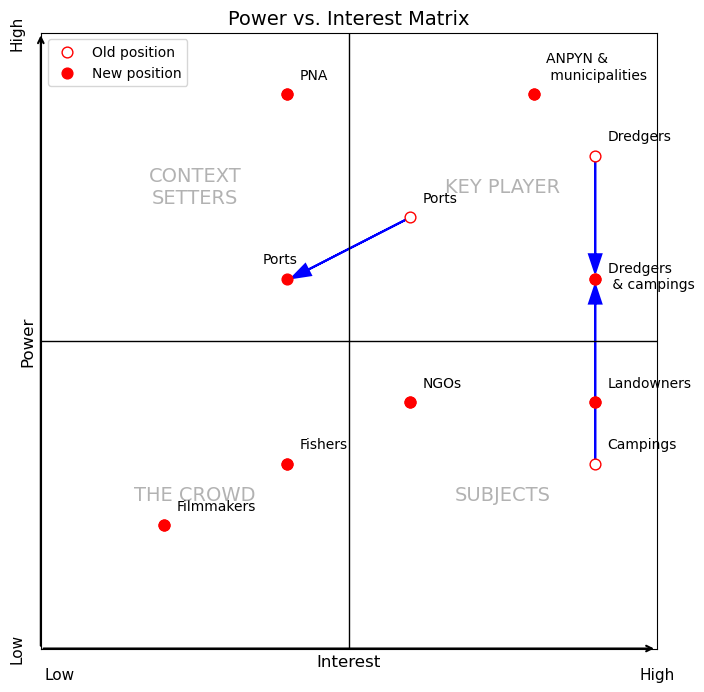
\includegraphics[width=0.70\linewidth]{figures/ch3/NewPowerVSInterest.png}
    \caption{Updated Power vs. Interest}
    \label{fig:power-interestNEW}
\end{figure}

\subsection{Power vs. Support-Opposition}
In figure \ref{fig:power-supportNEW}, the updated power vs. opposition-support-matrix can be found. The powers are updated in the same way as in figure \ref{fig:power-interestNEW} and the degree of opposition was changed for the landowners and campings. From the interviews, many concerns about the dredging operations arose, such as sound pollution and erosion. Many voiced their opposition to the dredging clearly, which is why these stakeholders were moved to the left on the opposition/support scale. For the dredgers and ports, the same degree of support still holds, for monetary reasons. The municipality is opposed to the dredging, as can be seen from the mayor's statements on the discontinuation of dredging.

\begin{figure}[H]
    \centering
    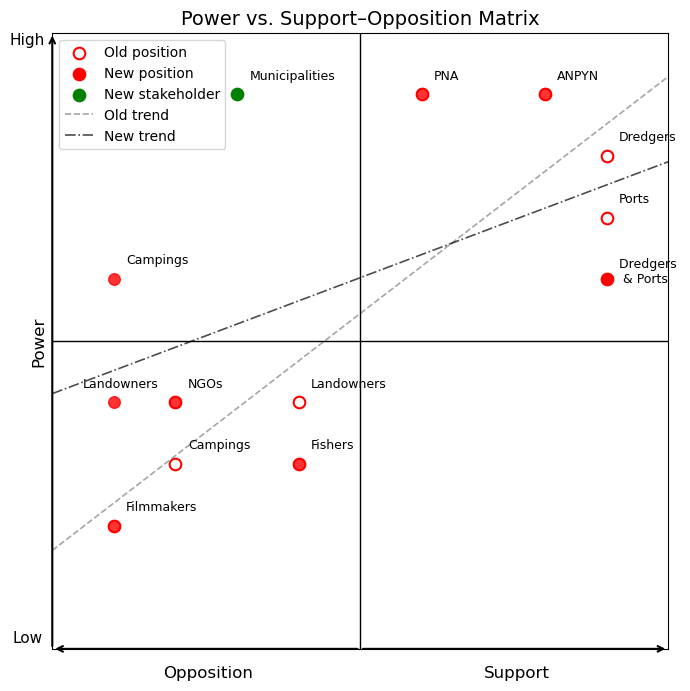
\includegraphics[width=0.70\linewidth]{figures/ch3/NewPowerVSSupport.png}
    \caption{Updated Power vs. Opposition-Support}
    \label{fig:power-supportNEW}
\end{figure}

In figure \ref{fig:power-supportNEW}, it can be seen that the new trend is flatter than the original one. This is a consequence of the fact that dredging operations have not increased in recent years, as opposed to the expectation, and have in fact been completely stopped on the Paraná-Ibicuy.

\section{Bank Erosion}